\documentclass[9pt, twocolumn]{article}
\newcommand\defaultstyle{\everymath{\displaystyle}}
\input{structure.tex}
\graphicspath{{./figures/}}
\usepackage{breqn,url,hyperref,listings,color,float, siunitx}
\usepackage[utf8]{inputenc}
\usepackage{tabularx}
\usepackage{graphicx}
\usepackage{adjustbox}
\hypersetup{
    colorlinks=true,
    linkcolor=blue,
    filecolor=magenta,
    urlcolor=cyan,
}
\urlstyle{same}

\definecolor{mygreen}{rgb}{0,0.6,0}
\definecolor{mygray}{rgb}{0.5,0.5,0.5}
\definecolor{mymauve}{rgb}{0.58,0,0.82}

\lstset{
    backgroundcolor=\color{white},   % choose the background color; you must add \usepackage{color} or \usepackage{xcolor}; should come as last argument
    %   basicstyle=\footnotesize,        % the size of the fonts that are used for the code
    breakatwhitespace=false,         % sets if automatic breaks should only happen at whitespace
    breaklines=true,                 % sets automatic line breaking
    captionpos=b,                    % sets the caption-position to bottom
    commentstyle=\color{mygreen},    % comment style
    deletekeywords={...},            % if you want to delete keywords from the given language
    escapeinside={\%*}{*)},          % if you want to add LaTeX within your code
    extendedchars=true,              % lets you use non-ASCII characters; for 8-bits encodings only, does not work with UTF-8
    firstnumber=1,                   % start line enumeration with line 1
    frame=single,	                   % adds a frame around the code
    keepspaces=false,                 % keeps spaces in text, useful for keeping indentation of code (possibly needs columns=flexible)
    keywordstyle=\color{blue},       % keyword style
    language=C,                 % the language of the code
    morekeywords={*,...},            % if you want to add more keywords to the set
    numbers=none,                    % where to put the line-numbers; possible values are (none, left, right)
    numbersep=5pt,                   % how far the line-numbers are from the code
    numberstyle=\tiny\color{mygray}, % the style that is used for the line-numbers
    rulecolor=\color{black},         % if not set, the frame-color may be changed on line-breaks within not-black text (e.g. comments (green here))
    showspaces=false,                % show spaces everywhere adding particular underscores; it overrides 'showstringspaces'
    showstringspaces=false,          % underline spaces within strings only
    showtabs=false,                  % show tabs within strings adding particular underscores
    stepnumber=2,                    % the step between two line-numbers. If it's 1, each line will be numbered
    stringstyle=\color{mymauve},     % string literal style
    tabsize=2,	                   % sets default tabsize to 2 spaces
    title=\lstname                   % show the filename of files included with \lstinputlisting; also try caption instead of title
}


\definecolor{codegray}{rgb}{0.5,0.5,0.5}
\definecolor{codepurple}{rgb}{0.58,0,0.82}
\definecolor{backcolour}{rgb}{0.95,0.95,0.92}
\lstdefinestyle{assembly}{
    backgroundcolor=\color{backcolour},   
    commentstyle=\color{codegray},
    keywordstyle=\color{blue},
    numberstyle=\tiny\color{codegray},
    stringstyle=\color{codepurple},
    basicstyle=\ttfamily\footnotesize,
    breakatwhitespace=false,         
    breaklines=true,                 
    captionpos=b,                    
    keepspaces=true,                 
    numbersep=5pt,                  
    showspaces=false,                
    showstringspaces=false,
    showtabs=false,                  
    tabsize=2,
    language=[x86masm]Assembler
}

% \newcommand{\hot}[1]{{\color{red} #1}}


\begin{document}
\defaultstyle
% \title{\vspace{-8ex}Homework 1 - Compiler Stages}
\title{\fontsize{17}{16}\selectfont
% Computer Architecture and Organization Project\\
\textbf{PipeViz: An Interactive Pipeline Simulator with LLM-Based Optimization}
%\\ \textbf{Univeristy of Notre Dame}
}

% \author{
% Laxminarayana Vadnala \textit{lvadnala@nd.edu}\\
% Patrick Do \textit{mdo23@nd.edu}\\
% Jude Lynch \textit{jlynch23@nd.edu}}

\author{
\begin{tabular}{ccc}
Laxminarayana Vadnala$^1$ & Patrick Do$^1$ & Jude Lynch$^1$ \\
\textit{lvadnala@nd.edu} & \textit{mdo23@nd.edu} & \textit{jlynch23@nd.edu}
\end{tabular}
\\[0.5em]
$^1$University of Notre Dame
}

\date{}
\maketitle
%---------------------------------------------------------------%
\section*{1. Abstract}
PipeViz is an interactive cycle-accurate pipeline simulation and visualization platform designed to analyze instruction-level execution behavior in modern processors. The system allows users to input C/C++ programs, compile them into AArch64 assembly, and simulate execution across multiple pipeline architectures including static in-order, scoreboarding, Tomasulo-based scheduling, superscalar, and out-of-order execution models. PipeViz automatically detects and visualizes pipeline hazards such as RAW, WAR, WAW, and structural hazards while presenting a cycle-by-cycle execution timeline through an interactive web interface.

In addition to simulation and visualization, PipeViz integrates a large language model (LLM)-based optimization assistant capable of analyzing source code, generated assembly, and pipeline execution traces to provide context-aware optimization recommendations. The system establishes an iterative workflow where users can observe pipeline inefficiencies, apply compiler or code-level optimizations, and compare the resulting execution behavior. Through multiple case studies involving loop unrolling and cache-aware matrix multiplication, we demonstrate how compiler transformations and LLM-guided optimizations influence hazard frequency, pipeline stalls, and instruction-level parallelism. PipeViz serves both as an educational platform for computer architecture and as an experimental framework for exploring the interaction between compiler optimizations and processor micro architecture. All code is open source and can be found here \cite{github-repo} and The "case\_studies" folder inside the "pipeviz" directory contains the results of the case studies conducted for this report can be found at this link \cite{case-studies}.
% kopje met bijbehorende titel; varianten: \subsection, \subsubsection
\section*{2. Introduction}

Modern processors achieve high performance through pipelined execution, allowing multiple instructions to overlap across different stages of execution. While pipelining significantly improves instruction throughput, it also introduces execution challenges caused by instruction dependencies, resource contention, and control-flow disruptions. Data hazards such as Read After Write (RAW), Write After Read (WAR), and Write After Write (WAW), along with structural hazards caused by limited hardware resources, can introduce stalls that reduce overall pipeline efficiency. Understanding how these hazards emerge from real programs is essential for studying processor microarchitecture, compiler optimizations, and instruction scheduling techniques.

Although pipeline behavior is widely taught in computer architecture courses, many existing educational tools rely on simplified examples or static diagrams that fail to demonstrate how modern compiled programs interact with realistic pipeline execution models. Additionally, the relationship between high-level source code, compiler-generated assembly, and cycle-level execution behavior is often difficult to visualize and reason about. Compiler optimizations such as loop unrolling, instruction scheduling, and vectorization can significantly alter instruction-level parallelism and hazard frequency, yet these effects are rarely observable in an integrated and interactive environment.

PipeViz was developed to address this gap by providing an end-to-end platform for pipeline simulation, hazard analysis, and optimization exploration. The system enables users to input C/C++ programs, compile them into AArch64 assembly using configurable compiler optimization settings, and simulate the resulting instructions across multiple execution models including static in-order pipelines, scoreboarding, Tomasulo-based scheduling, and out-of-order execution. During simulation, PipeViz tracks instruction progression cycle-by-cycle while detecting data and structural hazards and visualizing stalls directly within the pipeline timeline.

A major contribution of PipeViz is the integration of an LLM-driven optimization assistant that analyzes the generated assembly code and pipeline execution trace to provide context-aware explanations and optimization recommendations. Unlike traditional static code assistants, the LLM receives detailed micro architectural execution context, including hazard information, stall locations, compiler settings, and cycle-level pipeline state. This allows the assistant to reason about performance bottlenecks directly from observed execution behavior rather than relying solely on source-level heuristics.

The combination of cycle-accurate simulation, compiler experimentation, visualization, and AI-assisted reasoning transforms PipeViz into both an educational and experimental platform for studying processor execution behavior. Through a series of case studies involving loop unrolling and cache-aware matrix multiplication, this project demonstrates how pipeline-aware optimization strategies influence hazard frequency, instruction scheduling, and overall execution efficiency across different architectural models.

The primary objectives of this project are: \\
(1) Develop a cycle-accurate pipeline simulator capable of modeling multiple execution architectures. \\
(2) Detect and visualize RAW, WAR, WAW, and structural hazards during instruction execution. \\
(3) Enable users to experiment with compiler optimizations and observe their microarchitectural impact. \\
(4) Integrate an LLM assistant capable of analyzing pipeline execution traces and suggesting context-aware optimizations. \\
(5) Demonstrate the relationship between high-level code transformations and low-level processor behavior through interactive case studies. \\

\section*{3. Background and Related Concepts}

\begin{figure*}[t]
  \centering
  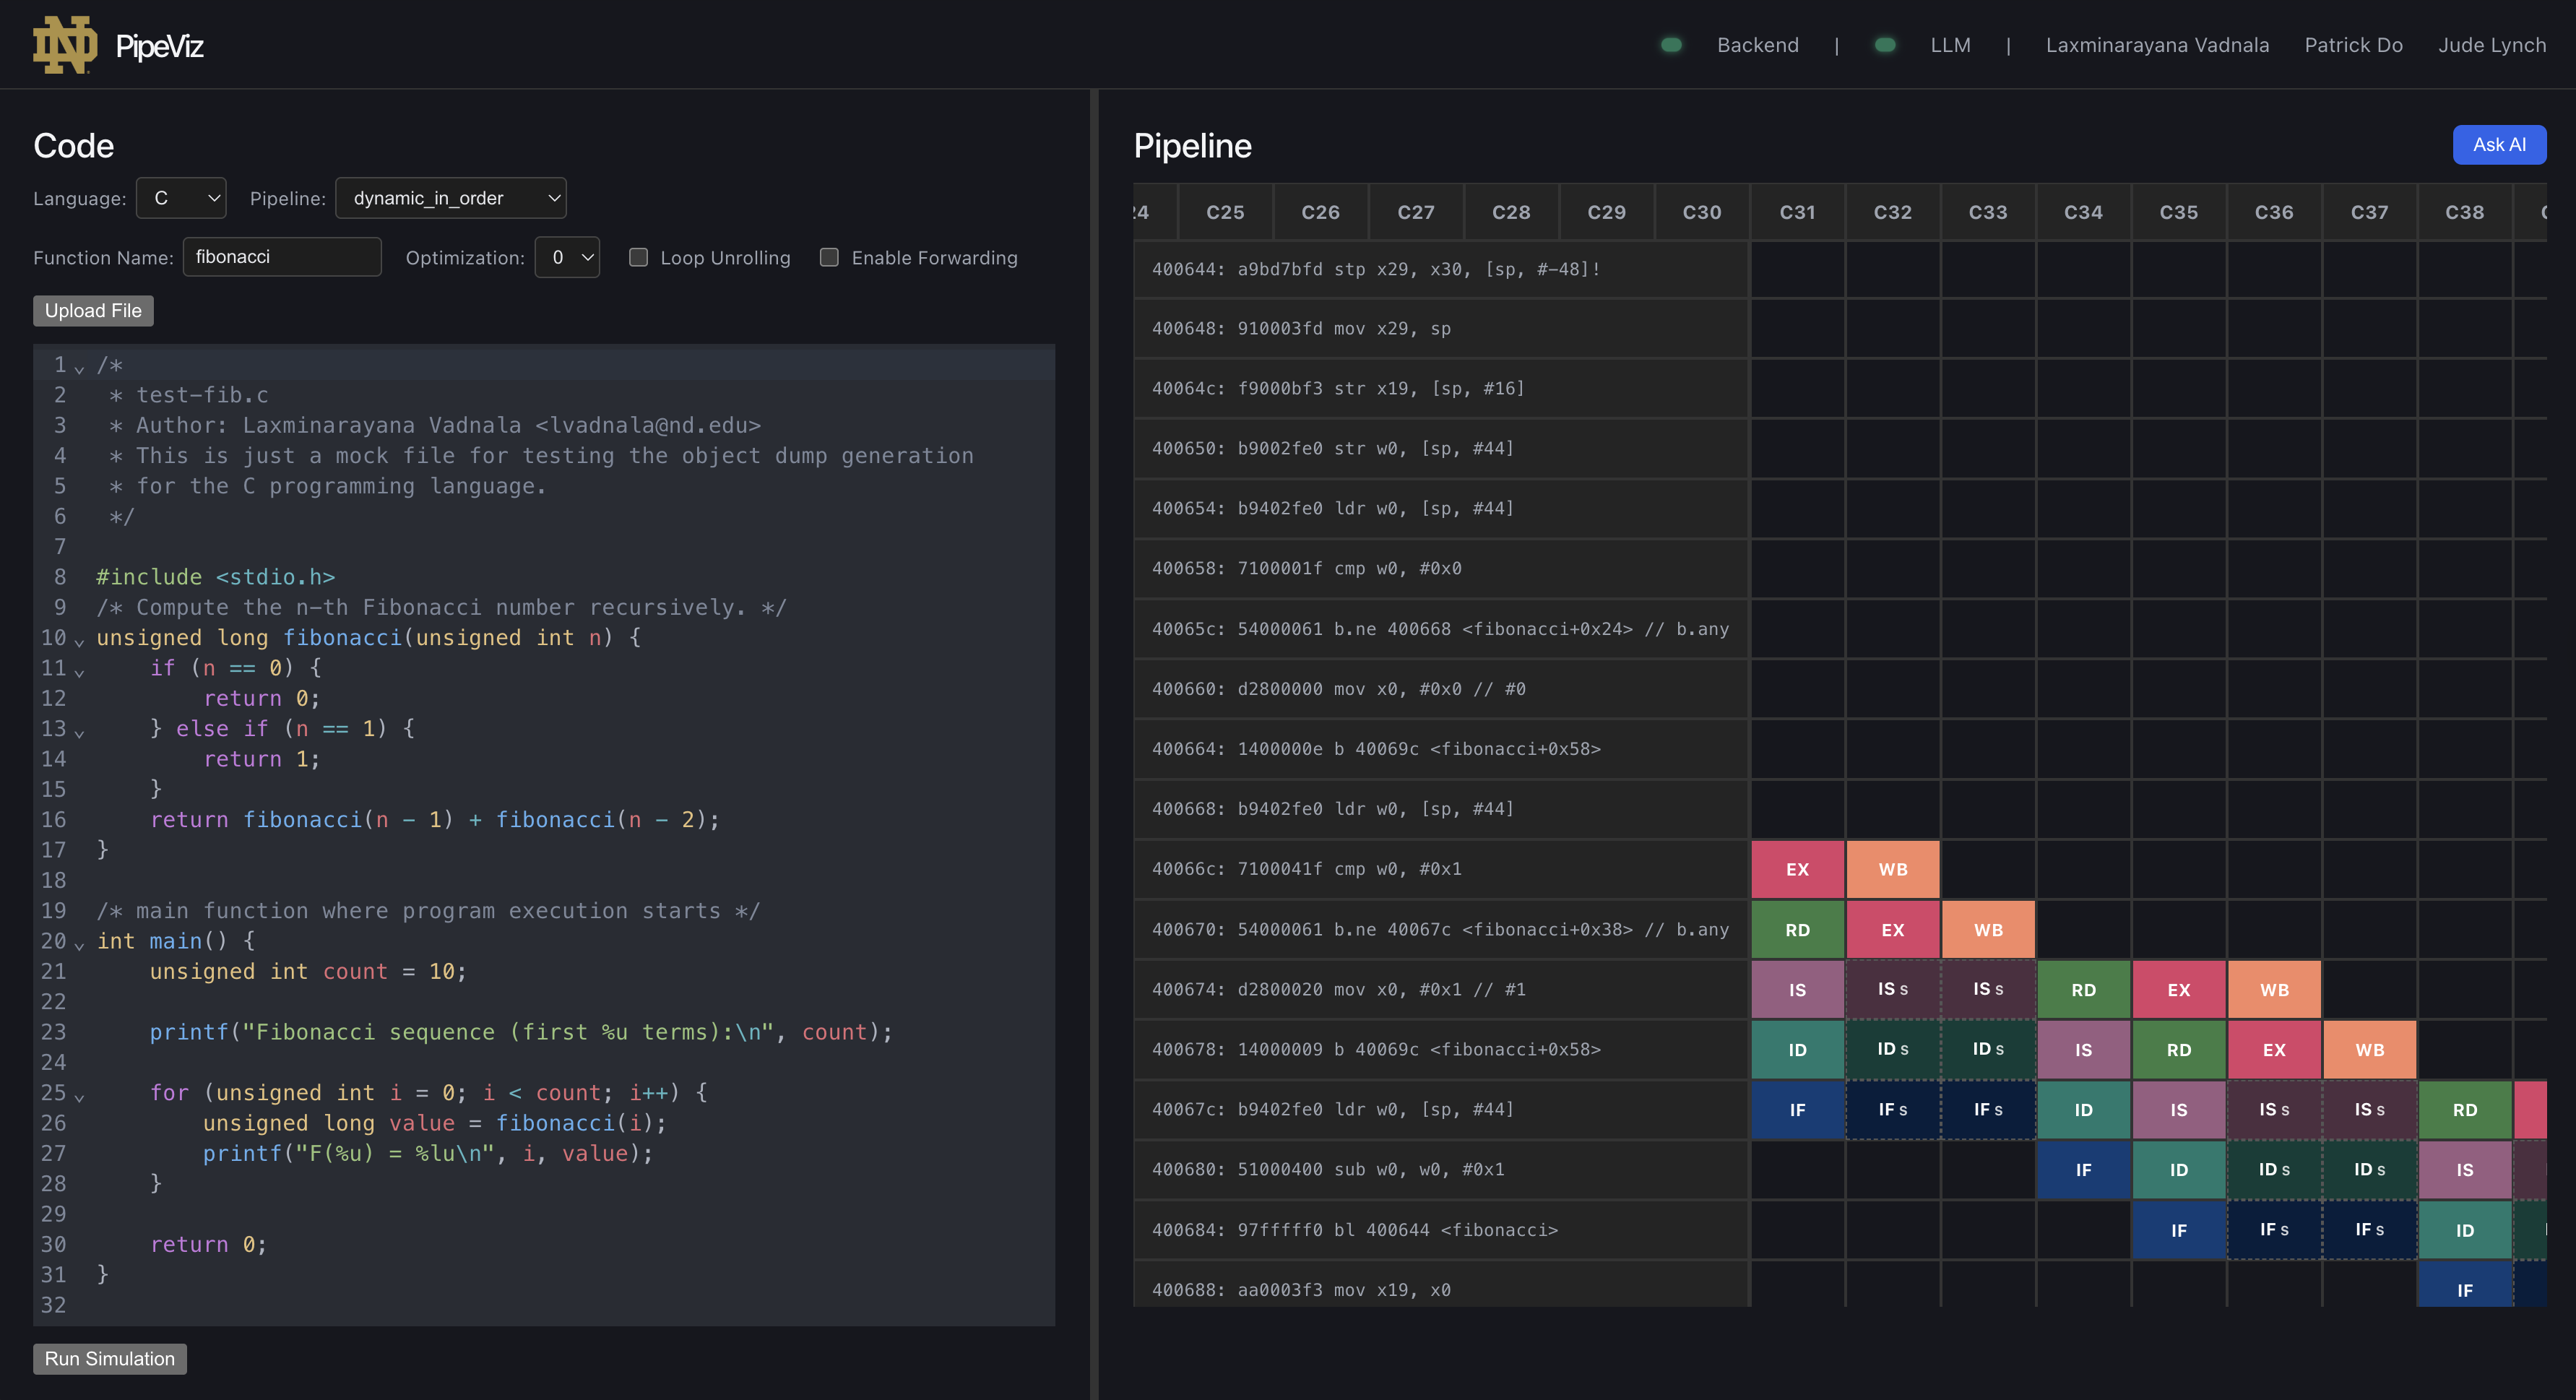
\includegraphics[width=\textwidth]{fig/pipeviz_interface.png}
  \vspace{-0.25in}
  \caption{The PipeViz user interface. The left panel provides a code editor with controls for language, pipeline model, target function, optimization level, loop unrolling, and data forwarding. The right panel displays the cycle-by-cycle pipeline execution table, where each row corresponds to an AArch64 instruction and each column represents a clock cycle. Stage labels are color-coded to indicate each instruction's progression through the pipeline.} 
  \label{fig:interface}
\end{figure*}

\subsection*{3.1 Pipeline Execution}
In a classic in-order pipeline, instructions progress through stages (fetch, decode, execute, memory, write back). Each cycle, ideally, one instruction advances to the next stage. Real execution deviates from this ideal due to dependencies and resource conflicts.


\subsection*{3.2 Data Hazards}
PipeViz detects three major data hazards: \\
(1) \textbf{RAW (Read After Write)}: An instruction reads a register before a previous instruction writes it. \\ 
(2) \textbf{WAR (Write After Read)}: An instruction writes a register before a previous instruction has read it.  \\
(3) \textbf{WAW (Write After Write)}: Two instructions write the same register in the wrong order.  \\


These hazards cause stalls when the pipeline must wait for a value to become available.

\subsection*{3.3 Structural Hazards}
Structural hazards occur when two or more instructions require the same hardware resource in the same cycle (e.g., memory access). This creates contention and stalls.

\subsection*{3.4 Compiler and Code Optimizations}
Compiler optimizations such as instruction scheduling, strength reduction, and loop unrolling often reduce hazards by increasing independence between instructions and improving utilization of pipeline stages. PipeViz leverages an LLM to suggest similar optimizations when a user observes frequent stalls.


\section*{4. System Overview}

\subsection*{4.1 PipeViz - Architecture}
% PipeViz is organized into three main components:

% \begin{enumerate}
%     \item \textbf{Frontend (pipeviz-ui)}: A React application that lets users input code, choose pipeline types, and view a cycle-by-cycle pipeline table.
%     \item \textbf{Backend (pipeviz)}: A FastAPI server that parses assembly, simulates pipeline execution, and detects hazards.
%     \item \textbf{LLM Assistant}: A prompt-driven optimization assistant that uses simulation output to propose improvements.
% \end{enumerate}

PipeViz is designed as a modular full-stack architecture that combines compilation infrastructure, pipeline simulation, visualization, and AI-assisted analysis into a unified workflow. The platform bridges the gap between high-level programming constructs and low-level processor execution by enabling users to move seamlessly from C/C++ source code to cycle-accurate pipeline analysis. The system architecture consists of three primary components: a React-based frontend visualization interface, a FastAPI-based \cite{fastapi} backend simulation engine, and an LLM-powered \cite{chatgpt, ollama} optimization assistant that performs context-aware reasoning over the generated execution data.

PipeViz is organized into three main components:

\textbf{Frontend (pipeviz-ui):} A React \cite{react, bun} application built with a syntax-highlighted code editor that lets users input C or C++ source code, select from seven pipeline models, configure compiler optimization levels (O0--O3), toggle loop unrolling and data forwarding, and view a cycle-by-cycle pipeline table. An integrated chat panel enables natural-language queries against the active simulation context. The full interface is shown in Figure~\ref{fig:interface}.

\textbf{Backend (pipeviz):} A FastAPI server that orchestrates four responsibilities: (1) invoking Docker-based \cite{docker} cross-compilation to generate AArch64 assembly, (2) parsing the resulting assembly into a structured instruction representation, (3) running a cycle-accurate simulation with hazard detection, and (4) persisting simulation context for downstream LLM queries.

\textbf{LLM Assistant:} A prompt-driven optimization assistant that uses a structured Jinja2 template containing the source code, generated assembly, and pipeline simulation table to query OpenAI's GPT-4o model, returning natural-language optimization recommendations grounded in the specific simulation output.

\subsection*{4.2 Workflow}
% The user workflow is:

% \begin{enumerate}
%     \item \textbf{Input source code} in the UI.  
%     \item \textbf{Assembly generation} (AArch64) using compiler tools.  
%     \item \textbf{Pipeline simulation} with hazard detection.  
%     \item \textbf{Visualization} of each instruction’s stage per cycle.  
%     \item \textbf{LLM analysis} using the prompt template, producing optimization suggestions.  
%     \item \textbf{Re-simulation} to compare hazards and stalls.
% \end{enumerate}

\textbf{Input:} The user enters source code in the editor and selects the target language (C or C++), pipeline model, compiler optimization level, and forwarding and loop unrolling options.

\textbf{Assembly generation:} The backend copies the source file and a language-specific Dockerfile into a temporary working directory, then invokes \texttt{docker build} with build arguments encoding the selected compiler flags. After the image builds, the container is instantiated, and the compiled AArch64 disassembly is extracted via \texttt{docker cp}. The container and image are cleaned up immediately after extraction.

\textbf{Function extraction:} A regular expression locates the target function symbol in the disassembly output and extracts its instruction lines, stopping at the next function boundary or section header.

\textbf{Pipeline simulation:} The simulator loads the parsed instruction stream and advances instructions through the pipeline cycle by cycle, recording a state snapshot at each cycle. Each snapshot captures stage occupancy, stall status, active hazards, and any forwarding paths.

\textbf{Visualization:} The simulation output is serialized as a JSON matrix---one row per instruction, one column per cycle---and rendered by the frontend as a color-coded grid. Each cell displays the stage name (e.g., \texttt{EX}) or \texttt{EX s} when a stall is active. Stage colors are consistent across all pipeline models: IF (blue), ID (teal), EX (red), MEM (yellow), WB (orange), IS (purple), and COM (brown).

\textbf{LLM analysis:} The simulation context---source code, assembly, pipeline table, and prior questions---is persisted and passed to the LLM assistant when the user submits a natural-language query via the chat panel. The model returns an optimization recommendation tied to the observed hazards and stall patterns.

\textbf{Re-simulation:} The user can apply the suggested changes and re-submit the code, enabling direct before-and-after comparison of stall counts and hazard frequency across pipeline models.
\section*{5. Pipeline Simulation Design}
% The simulator is rule-based and implements multiple pipeline models:

% \begin{enumerate}
% \item Static in-order  
% \item Scoreboard  
% \item Dynamic in-order  
% \item In-order superscalar  
% \item Tomasulo  
% \item VLIW  
% \item Out-of-order  
% \end{enumerate}

% The simulator processes instructions cycle by cycle, tracks each instruction state, and detects hazards based on current stage occupancy and register dependencies. When hazards are present, stages are stalled and displayed with a `[STALL]` marker in the visualization.

% Key design elements:

% \begin{enumerate}
% \item \textbf{Instruction parsing} from ARM64 assembly (\textit{pipeline_base.py}).
% \item \textbf{Hazard detection} through the \textit{HazardDetector} class.
% \item \textbf{Stage modeling} through pipeline enums, allowing multiple pipeline types.
% \item \textbf{Cycle-level state snapshots} stored as \textit{PipelineState}.
% \end{enumerate}

The simulator is rule-based and implements seven pipeline models. Each model is defined as a typed enumeration that declares its ordered stages and annotates which stages are susceptible to each hazard type. This design allows the simulation and hazard detection logic to operate generically across all models without branching on pipeline type.


\textbf{Static In-Order:} A classic five-stage pipeline (IF $\to$ ID $\to$ EX $\to$ MEM $\to$ WB). RAW hazards are detected at the decode stage, structural hazards at decode, execute, and memory, and WAW hazards at writeback. This model produces the highest stall counts and serves as the performance baseline.

\textbf{Scoreboard:} A five-stage model (IF $\to$ IS $\to$ RD $\to$ EX $\to$ WB) that separates instruction issue from operand read. RAW hazards are detected at the read-operands stage, and structural hazards at issue and execute. WAW hazards are flagged at issue because register renaming is not yet applied.

\textbf{Dynamic In-Order:} A six-stage extension (IF $\to$ ID $\to$ IS $\to$ RD $\to$ EX $\to$ WB) that adds explicit decode and issue stages, providing finer-grained control over dispatch logic.

\textbf{In-Order Superscalar:} A seven-stage pipeline (IF $\to$ ID $\to$ IS $\to$ EX $\to$ MEM $\to$ WB $\to$ COM) that adds a commit stage. Multiple instructions can be in flight simultaneously, but issue order is preserved and instructions retire in program order.

\textbf{VLIW (Very Long Instruction Word):} A five-stage model structurally identical to the static in-order pipeline, but with all hazard-prone stage lists empty. Hazard avoidance is assumed to be handled entirely at compile time, with the compiler or programmer responsible for packing independent instructions into VLIW bundles.

\textbf{Tomasulo:} A five-stage out-of-order model (IF $\to$ IS $\to$ EX $\to$ WB $\to$ COM) that models reservation stations and register renaming. WAR and WAW hazards are eliminated through renaming. RAW hazards are resolved via result tagging rather than stalling. Structural hazards remain possible when reservation stations or functional units are fully occupied.

\textbf{Out-of-Order:} The most aggressive model, with six stages (IF $\to$ IS $\to$ RO $\to$ EX $\to$ WB $\to$ COM), where RO represents the reorder buffer (ROB) that enforces in-order retirement. All data hazards are eliminated via register renaming; only structural hazards remain, possible at issue, ROB, execute, and writeback.
\section*{6. LLM Integration}

% PipeViz includes a structured prompt template (\textit{prompt_template.md.j2}) that feeds the LLM:

% \begin{enumerate}
%     \item Source code  
%     \item Generated assembly  
%     \item Pipeline stages  
%     \item Pipeline simulation table (with stalls)  
% \end{enumerate}

% The LLM is asked to:
% \begin{enumerate}
%     \item Identify inefficiencies in the pipeline output.
%     \item Explain the hazards causing stalls.
%     \item Suggest optimizations (e.g., loop unrolling, reordering, reducing dependencies).
% \end{enumerate}

% This creates a human-readable analysis layer on top of the simulator output.

One of the central innovations of PipeViz is the integration of a large language model (LLM) as a pipeline-aware optimization assistant. Traditional optimization assistants typically operate only on source code and lack visibility into actual processor execution behavior. In contrast, PipeViz provides the LLM with detailed micro architectural context including generated AArch64 assembly, detected hazards, compiler optimization settings, and cycle-by-cycle pipeline traces. This enables the assistant to reason about performance bottlenecks using concrete execution evidence rather than generalized programming heuristics.

The LLM integration transforms PipeViz from a passive visualization tool into an interactive architectural analysis environment. Users can query the assistant about specific stalls, dependencies, or execution inefficiencies and receive explanations grounded in the observed pipeline behavior. The assistant can also suggest optimizations such as loop unrolling, instruction reordering, register reuse reduction, and cache-aware restructuring, allowing users to iteratively refine their programs and immediately validate the impact through re-simulation.

\subsection*{6.1 Prompt Design}
The LLM receives a structured prompt rendered from a Jinja2 template that assembles four categories of context: (1) the model is assigned the role of a computer architecture expert and instructed not to infer values not present in the provided data; (2) the full source code of the simulated function is included alongside all relevant compilation and simulation parameters; (3) the ARM64 disassembly produced by the compilation step is provided in full, allowing the model to reason at the instruction level about register dependencies and memory access patterns; and (4) the cycle-by-cycle pipeline execution table is included with stall stages annotated.

This structured context grounds the model's suggestions in the actual observed pipeline behavior rather than general heuristics, reducing the risk of generic or inapplicable recommendations.

\subsection*{6.2 Interaction Model}
The assistant supports a multi-turn conversation within a simulation session. Each query is associated with a persistent workflow identifier that links the question to the corresponding simulation context. Prior questions are accumulated and included in subsequent prompts, allowing the model to maintain coherence across follow-up queries without requiring the user to restate context. A prompt length limit of 75,000 tokens is enforced to prevent context window overflow for programs with large assembly outputs.

\subsection*{6.3 Optimization Suggestions}

The LLM is asked to perform three tasks given the simulation output:\\
(1) Identify inefficiencies in the pipeline table, such as repeated stalls or high-latency instruction sequences. \\
(2) Explain the root cause of detected hazards in terms of register dependencies or resource contention between specific instructions.\\
(3) Propose concrete optimizations at the source code or assembly level, including techniques such as instruction reordering, loop unrolling, strength reduction, or reducing register dependencies to allow better pipeline utilization.

The suggestions are returned as natural-language text and displayed in the chat panel. The user can then apply the changes, resubmit the code, and observe the impact on stall counts and hazard frequency in the updated simulation. This creates an iterative refinement loop: code $\to$ pipeline $\to$ LLM analysis $\to$ optimization $\to$ improved pipeline.
\section*{7. Case Studies}

To evaluate the effectiveness of PipeViz, we conducted multiple case studies exploring how compiler optimizations and LLM-guided transformations affect pipeline execution behavior. These studies focus on analyzing hazard frequency, instruction scheduling efficiency, memory access patterns, and instruction-level parallelism across different execution models. By combining cycle-accurate simulation with contextual LLM analysis, the experiments demonstrate how PipeViz can be used both as an educational visualization platform and as a practical micro-architectural optimization tool.

The case studies specifically investigate two optimization scenarios: cache-aware matrix multiplication and compiler-assisted loop unrolling. In each experiment, the system compares baseline implementations against optimized variants while visualizing the resulting changes in hazard behavior, pipeline stalls, and execution overlap. These experiments highlight the relationship between high-level algorithmic transformations and low-level processor execution characteristics.

\subsection*{Case Study 1. LLM-Driven Cache Optimization and Pipeline Analysis for Matrix Multiplication}

\textbf{Methodology and Experimental Setup.} This case study demonstrates the integration of LLM-assisted code optimization with detailed micro-architectural pipeline simulation using the PipeViz tool. A baseline matrix multiplication implementation (\texttt{64$\times$64} double-precision matrices) was submitted to the pipeline visualization system configured with a static in-order execution model targeting \texttt{AArch64} architecture. The original code employed a triple-nested loop structure (\texttt{i-j-k} ordering) with no explicit cache optimization. Here is the User code input:

\begin{lstlisting}[language=C, basicstyle=\ttfamily\scriptsize, tabsize=2]
#include <stdio.h>
#include <stdlib.h>
#include <string.h>
#include <time.h>

#define N 64      // Matrix size
#define B 8       // Blocking factor (cache line size consideration)

void matrix_multiply(double x[N][N], double y[N][N], double z[N][N]) {
    for (int i = 0; i < N; i++) {
        for (int j = 0; j < N; j++) {
            for (int k = 0; k < N; k++) {
                x[i][j] = x[i][j] + y[i][k] * z[k][j];
            }
        }
    }
}

// Initialize matrices
void init_matrices(double x[N][N], double y[N][N], double z[N][N]) {
    for (int i = 0; i < N; i++) {
        for (int j = 0; j < N; j++) {
            x[i][j] = 0.0;
            y[i][j] = (double)(i * N + j);
            z[i][j] = (double)((i + j) % N);
        }
    }
}

int main() {
    double (*x)[N] = malloc(sizeof(double) * N * N);
    double (*y)[N] = malloc(sizeof(double) * N * N);
    double (*z)[N] = malloc(sizeof(double) * N * N);
    
    if (!x || !y || !z) {
        fprintf(stderr, "Memory allocation failed\n");
        return 1;
    }

    init_matrices(x, y, z);
    
    // Run blocked version
    matrix_multiply(x, y, z);
    
    // Print result sample
    printf("Result[0][0] = %f\n", x[0][0]);
    printf("Result[5][5] = %f\n", x[5][5]);
    
    free(x);
    free(y);
    free(z);
    
    return 0;
}
\end{lstlisting}

After compilation with user-specified optimization flags, the generated assembly code was extracted and simulated through the five-stage pipeline (\texttt{IF}$\rightarrow$\texttt{ID}$\rightarrow$\texttt{EX}$\rightarrow$\texttt{MEM}$\rightarrow$\texttt{WB}), with the tool automatically identifying and visualizing data hazards (\texttt{RAW}, \texttt{WAR}, \texttt{WAW}) and structural hazards at each clock cycle. This baseline simulation established performance metrics, including pipeline stalls, bubble insertion patterns, and memory access characteristics that would serve as the comparison point for optimization. Here is the figure~\ref{fig:cycle-instructions} that shows the "\texttt{Static in order}" cycle-by-cycle instructions.

\begin{figure*}[t]
  \centering
  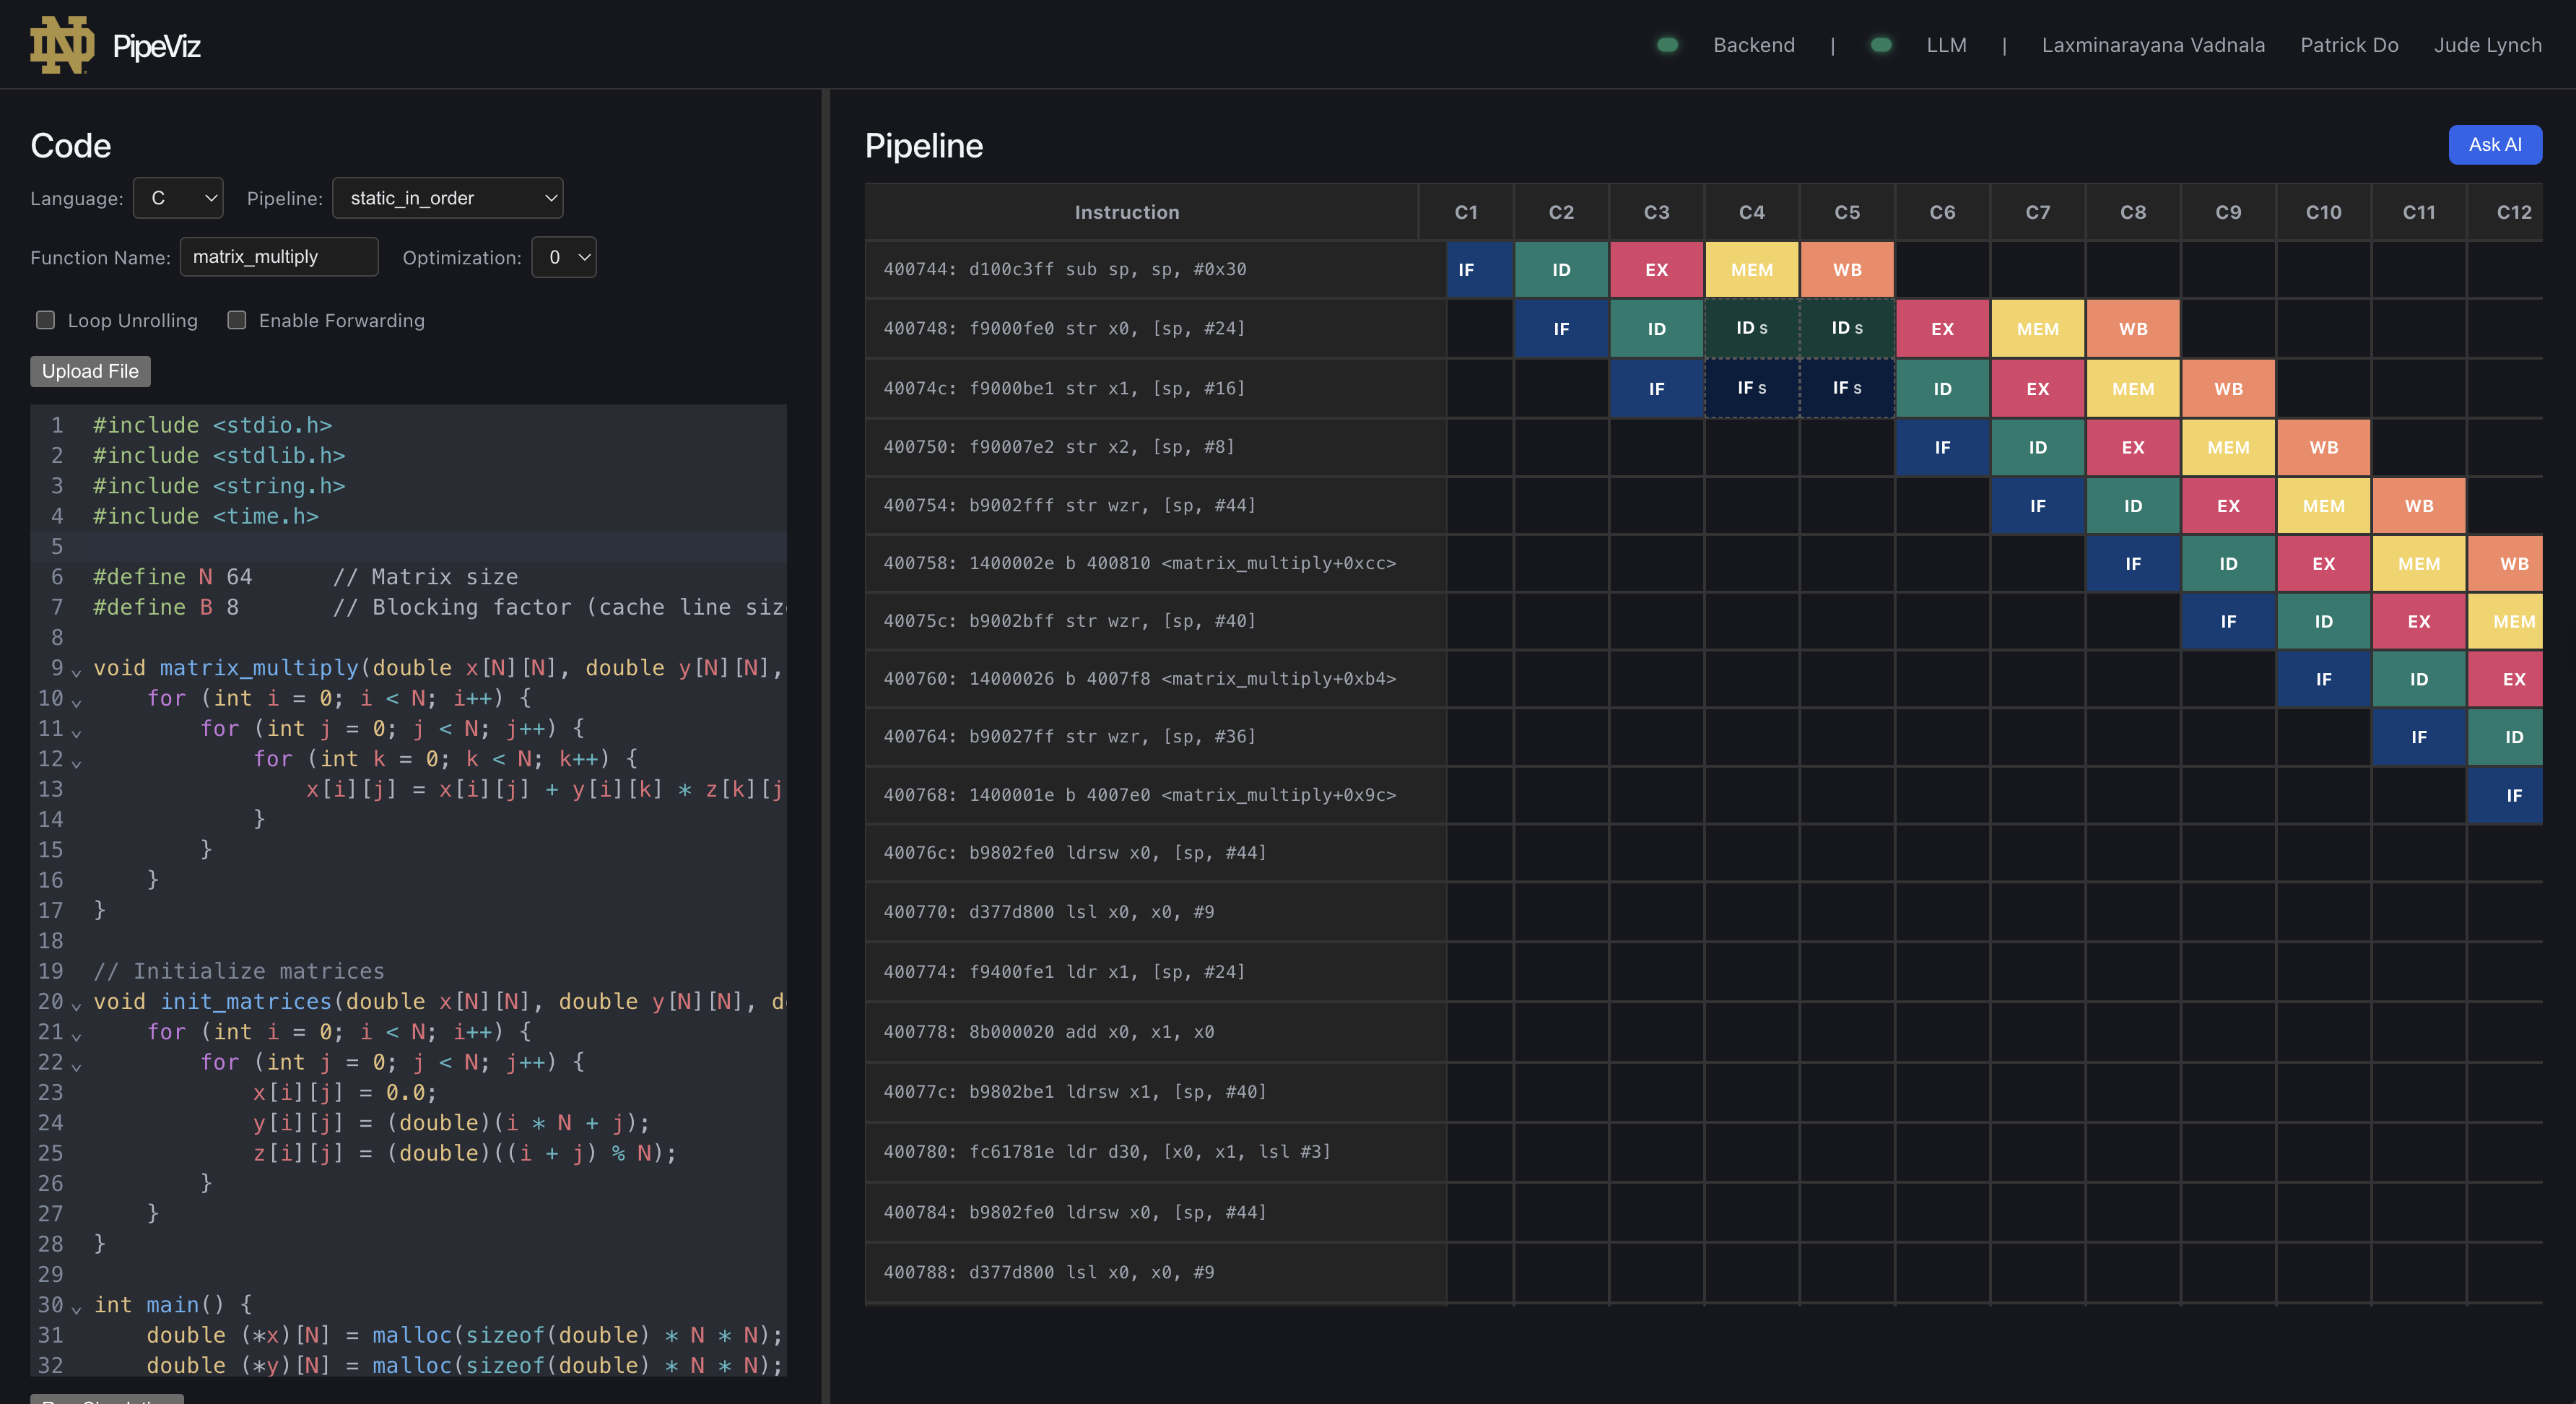
\includegraphics[width=\textwidth]{fig/cycle-instructions.png}
  \vspace{-0.25in}
  \caption{The PipeViz user interface showing the cycle-by-cycle instructions. This run refers to the matrix multiplication case study.}
  \label{fig:cycle-instructions}
\end{figure*}

\textbf{LLM-Suggested Optimization Strategy.} The integrated LLM-based chatbot was provided with the complete context of the baseline implementation—including the original C source code, generated \texttt{AArch64} assembly, and the detailed pipeline simulation data showing hazard patterns and execution bottlenecks. Analyzing this micro architectural feedback, the LLM proposed a cache-blocked (tiled) matrix multiplication algorithm using a blocking factor of \texttt{8} (matching the original \texttt{B} constant). The optimized implementation introduces an outer tile-iteration structure (\texttt{ii-jj-kk} loops) that partitions the matrix operations into \texttt{8$\times$8} subblocks, with inner loops (\texttt{i-j-k}) operating within each tile. Critically, the optimization accumulates partial results in a scalar temporary (\texttt{sum}) before writing back to the output matrix, reducing the number of load-modify-store operations per element. This restructuring aims to improve spatial and temporal locality, keeping working sets within \texttt{L1} cache boundaries and potentially reducing memory-stage stalls observed in the baseline pipeline simulation.

Here is the LLM suggested C code:

% \begin{lstlisting}[language=C, basicstyle=\footnotesize]
% #define N 64
% #define B 8

% void matrix_multiply(double x[N][N],
%                     double y[N][N],
%                     double z[N][N]) {

%     for (int ii = 0; ii < N; ii += B) {
%         for (int jj = 0; jj < N; jj += B) {
%             for (int kk = 0; kk < N; kk += B) {

%                 for (int i = ii; i < ii + B; i++) {

%                     for (int j = jj; j < jj + B; j++) {

%                         double sum = x[i][j];

%                         for (int k = kk; k < kk + B; k++) {
%                             sum += y[i][k] * z[k][j];
%                         }

%                         x[i][j] = sum;
%                     }
%                 }
%             }
%         }
%     }
% }
% \end{lstlisting}

\begin{lstlisting}[language=C, basicstyle=\ttfamily\scriptsize, tabsize=2]
#define N 64
#define B 8

void matrix_multiply(double x[N][N], double y[N][N], double z[N][N]) {
  for (int ii = 0; ii < N; ii += B) {
    for (int jj = 0; jj < N; jj += B) {
      for (int kk = 0; kk < N; kk += B) {
        for (int i = ii; i < ii + B; i++) {
          for (int j = jj; j < jj + B; j++) {
            double sum = x[i][j];
            for (int k = kk; k < kk + B; k++) {
              sum += y[i][k] * z[k][j];
            }
            x[i][j] = sum;
          }
        }
      }
    }
  }
}
\end{lstlisting}

\begin{figure*}[t]
  \centering
  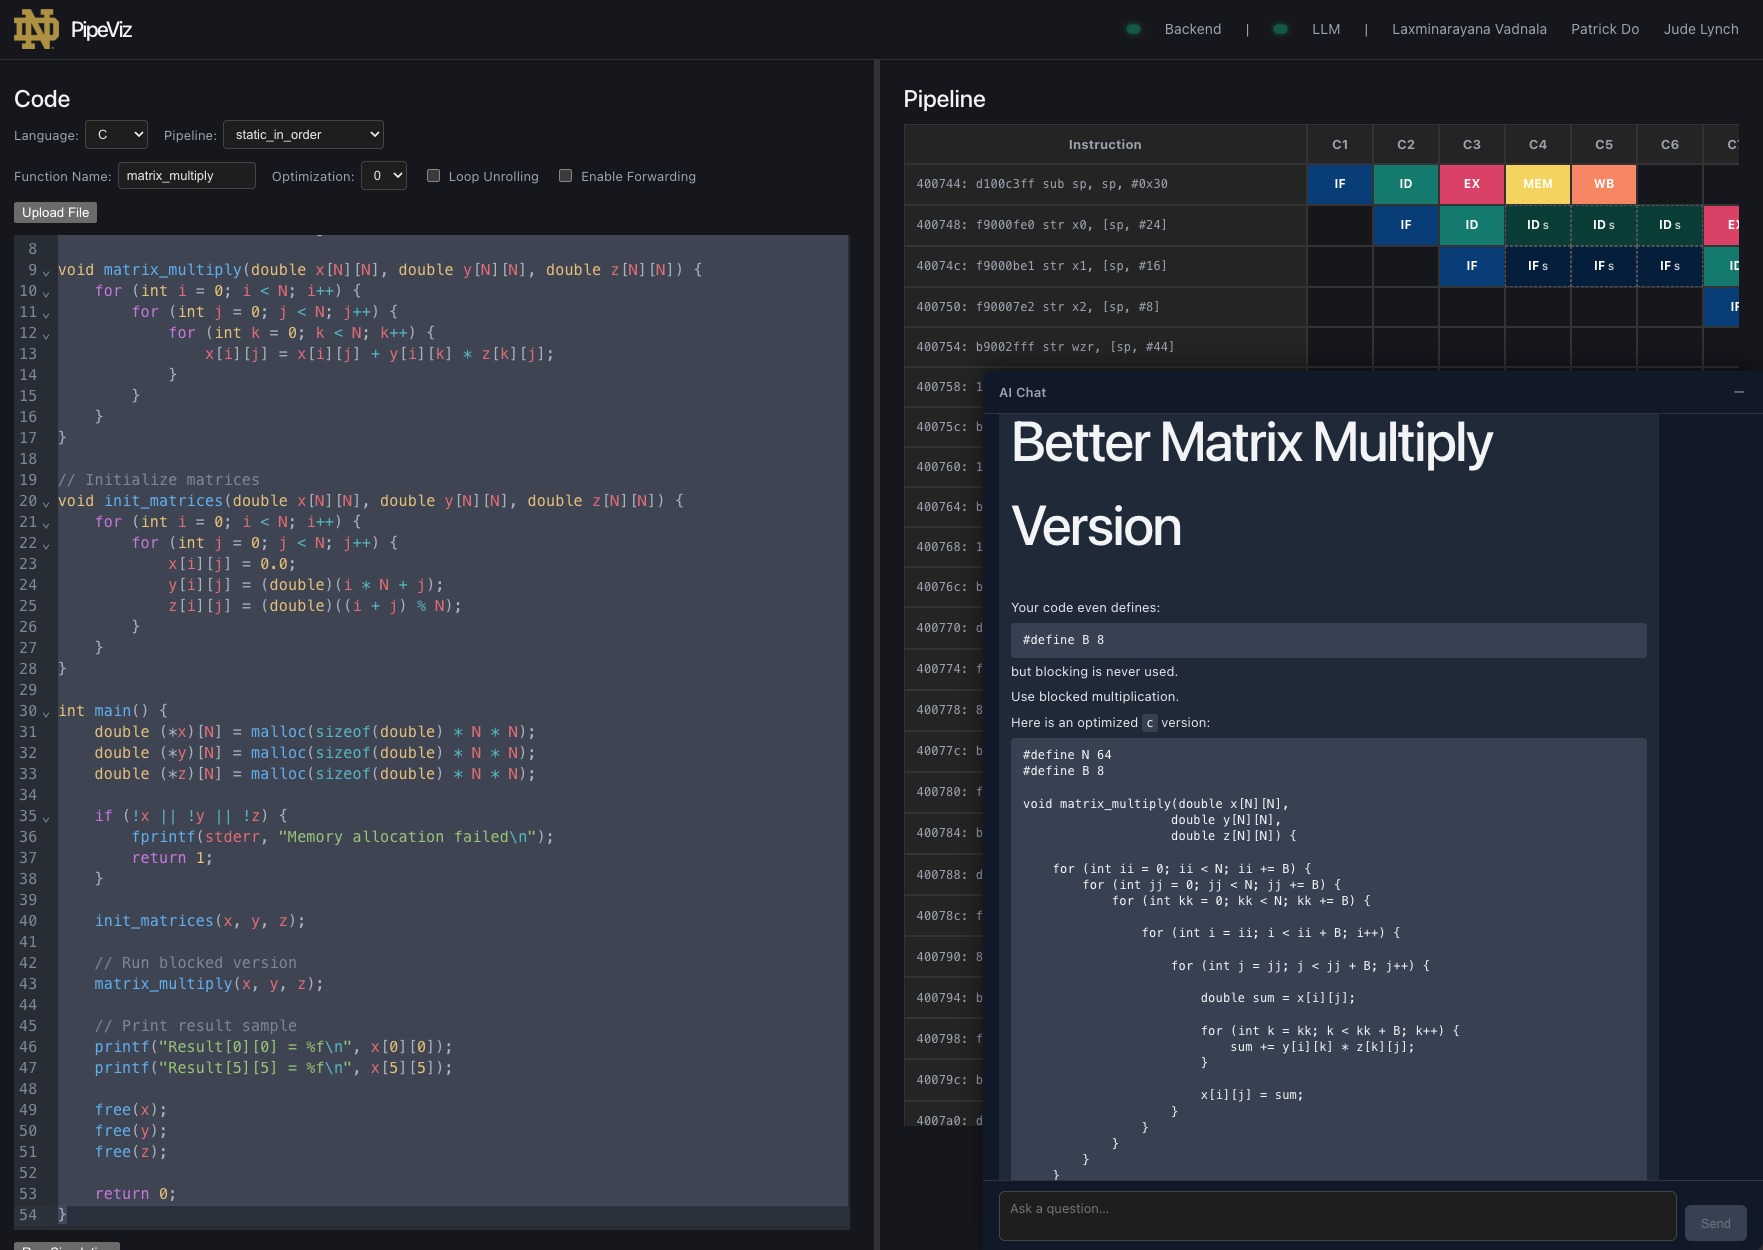
\includegraphics[width=\textwidth]{fig/LLM-matrix-multiply-response.png}
  \vspace{-0.25in}
  \caption{The PipeViz user interface showing the user code and optimal code suggested by the LLM based on the context fed to it while generating the response.}
  \label{fig:llm-matrix-response}
\end{figure*}

\textbf{Pipeline Simulation Analysis and Micro architectural Insights.} When both implementations were processed through identical pipeline configurations (static in-order, same compiler flags), the PipeViz tool revealed distinct hazard patterns and execution characteristics. The baseline implementation exhibited frequent \texttt{RAW} hazards in the innermost \texttt{k}-loop, where the load of \texttt{x[i][j]} for accumulation created dependencies with subsequent stores, forcing pipeline stalls in the \texttt{MEM} stage. The blocked version's use of a register-resident accumulator (\texttt{sum}) reduced these memory-dependent \texttt{RAW} hazards within each tile's inner loop, allowing more instruction-level parallelism despite the static in-order execution constraint. The visualization also highlighted differences in memory access patterns: the original code's column-major access to \texttt{z[k][j]} caused poor cache behavior visible as structural hazards on the memory unit, while the blocked version's smaller working set improved cache line utilization. The tool's ability to display these hazards alongside the assembly code enabled direct correlation between high-level algorithmic choices and low-level execution behavior. Here is the figure~\ref{fig:llm-matrix-response} shows the response from LLM

\textbf{Impact and Validation of LLM-Assisted Micro architectural Optimization.} This case study validates the efficacy of combining LLM code optimization with detailed pipeline simulation feedback. By providing the LLM with both the source code and the microarchitectural execution trace—including specific hazard locations and pipeline stall patterns—the system enabled context-aware optimization that addressed observable performance bottlenecks rather than applying generic transformations. The blocking optimization suggested by the LLM directly targeted the memory-hierarchy issues visible in the baseline pipeline simulation, demonstrating that language models can effectively reason about low-level performance when given appropriate micro-architectural context. This integrated approach creates a feedback loop where pipeline simulation informs optimization, and re-simulation validates improvements, providing developers with both actionable code changes and detailed visual evidence of their micro-architectural impact. The PipeViz tool thus serves not only as an educational platform for understanding pipeline behavior but as a practical optimization assistant capable of bridging the gap between high-level algorithm design and hardware execution reality.


\subsection*{Case Study 2. Loop-Unrolling Case Study in PipeViz}

% For the loop-unrolling case study, we used the same simple nested-loop kernel in C, compiled to AArch64 under the static in order pipeline model, and then compared two runs: one compiled with the loop-unrolling option enabled (vectorized, long straight-line kernel) and one compiled without loop unrolling (shorter loop body that iterates more frequently). In both cases, PipeViz ingests the generated assembly, simulates the program cycle by cycle through the five-stage pipeline (IF–ID–EX–MEM–WB), and records all observed RAW, WAR, WAW, and structural hazards directly from the simulated trace.
% Here is the code we have used for the experiment.

% \begin{lstlisting}[language=C, basicstyle=\ttfamily\scriptsize, tabsize=2]
% #include <stdio.h>

% int main(void) {
%     int n = 1000;
%     int sum = 0;
%     for (int i = 0; i < n; i++) {
%         for (int j = 0; j < n; j++) {
%             sum += i + j;
%         }
%     }
%     printf("sum = %d\n", sum);
%     return 0;
% }
% \end{lstlisting}


% In the non-unrolled version, the inner loop body is relatively compact: each iteration executes a handful of vector ADD and MLA instructions and then branches back. The pipeline simulation shows a dense chain of RAW dependencies along the main accumulation register ("v30") and the temporary vector registers ("v26", "v25", "v31"). Because we model a simple static in-order pipeline with ideal forwarding, most of these RAW dependencies do not show up as explicit stall cycles, but they still constrain the schedule: many instructions consume values that are produced only one or two cycles earlier, leaving very little slack. As a result, the pipeline has limited opportunity to overlap independent work. At the tail of the function, we also see a visible RAW stall between the horizontal reduction ("addv s31, v30.4s" or "addv s29, v1.4s") and the scalar move ("fmov w1, s31/s29"), which forces the ID stage of "fmov" to wait one cycle until the reduction result is written back. Finally, there is a structural hazard on the call to "printf": the branch-and-link ("bl") occupies the fetch path and produces an "IF[STALL]" in the next cycle while the pipeline redirects control flow.

%  In the unrolled configuration, the compiler expands the inner computation into a much longer straight-line vector kernel. We now see a wide strip of ADD and MLA operations over many different vector registers ("v17", "v19", "v20", "v21", "v22", "v23", "v24", "v25", "v26", "v30", "v31", etc.), rather than repeatedly executing a very short body. PipeViz’s hazard analysis shows that this transformation reduces the effective density of RAW hazards in the core loop: there are still true dependencies, but more of them are spread across independent accumulators instead of being tightly chained on a single register every few cycles. Because the static in-order model can now interleave independent vector operations, many potential RAW conflicts are naturally overlapped in EX, so we do not introduce additional stall cycles in the loop body. In other words, after loop unrolling, we are able to lower the number of stall-inducing RAW hazards in the hot loop, even though the total number of dynamic arithmetic instructions increases.


% The "-O2" compilation (first assembly) executes a compact loop that increments the counter by 1 (add w0, w0, \#0x1 at offset 0x56c) and performs minimal vector operations per iteration, creating a tight 20-byte loop body that branches back frequently. In contrast, the -O2 -funroll-loops version (second assembly) unrolls the loop to increment the counter by 10 (add w0, w0, \#0xa at offset 0x56c), expanding the loop body to ~208 bytes with multiple vector operations (movi, add, mla, mov instructions on vector registers v1-v31) that handle 10 loop iterations worth of computation in each iteration. This trade-off reduces branch prediction pressure and loop overhead—the branch penalty is paid only once per 10 iterations instead of per iteration—but at the cost of increased code size (0x148 bytes vs 0x74 bytes for main) and higher instruction-level parallelism demands. The unrolled version allows the CPU to exploit more parallelism across multiple independent vector operations within a single iteration, reducing data dependency stalls typical of tight loops, making it ideal for demonstrating how compiler optimizations interact with pipeline architecture in your project evaluation.

% Crucially, loop unrolling does not change the structural side of the pipeline in this experiment. In both the unrolled and non-unrolled traces, the only prominent structural event is still the call to "printf", which causes the same fetch-stage stall pattern around the "bl" instruction. The pipeline model still has a single branch back to the loop head and a single function call in the epilogue; unrolling modifies the amount of work done between branches, but it does not introduce or remove contended structural resources. As a result, the structural hazard profile remains essentially identical across the two runs: the same "IF[STALL]" at the call site and no new structural conflicts elsewhere.

% Finally, the end-of-loop reduction sequence behaves the same way in both configurations: the "addv" that collapses the vector accumulator into a scalar is immediately followed by "fmov" to move that scalar into a general-purpose register. In our static in-order model, this pair continues to manifest as a single RAW-induced stall at the ID stage of "fmov", regardless of whether the loop body was unrolled. The key impact of loop unrolling, therefore, is not to eliminate that final RAW hazard or to change structural hazards, but to reshape the inner-loop schedule so that more of the arithmetic is independent and can be overlapped, which shows up in PipeViz as fewer RAW-induced stalls in the hot region of the pipeline while leaving the structural hazard behavior effectively unchanged.

\textbf{Methodology and Experimental Setup.} This case study examines how the compiler optimization flag \texttt{-funroll-loops} affects pipeline execution behavior by comparing two compiled variants of the same nested-loop kernel. A simple double-nested summation program was submitted to the PipeViz pipeline visualization system under two configurations: a baseline compiled with \texttt{-O2} and an optimized variant compiled with \texttt{-O2 -funroll-loops}, both targeting AArch64 architecture. In each case, the generated assembly was simulated through the five-stage static in-order pipeline (IF$\rightarrow$ID$\rightarrow$EX$\rightarrow$MEM$\rightarrow$WB), with PipeViz automatically identifying and recording all RAW, WAR, WAW, and structural hazards at each clock cycle. The baseline simulation established a reference point for hazard frequency, stall patterns, and instruction scheduling behavior against which the unrolled variant could be directly compared. Here is the C source code used for the experiment:

\begin{lstlisting}[language=C, basicstyle=\ttfamily\scriptsize, tabsize=2]
#include <stdio.h>

int main(void) {
    int n = 1000;
    int sum = 0;
    for (int i = 0; i < n; i++) {
        for (int j = 0; j < n; j++) {
            sum += i + j;
        }
    }
    printf("sum = %d\n", sum);
    return 0;
}
\end{lstlisting}

\textbf{Compiler Loop Unrolling Strategy.} The \texttt{-funroll-loops} flag instructs the compiler to expand the inner loop body so that multiple iterations of computation are performed per loop cycle. In the baseline \texttt{-O2} compilation, the inner loop body is compact---approximately 0x74 bytes for \texttt{main}---incrementing the loop counter by one (\texttt{add w0, w0, \#0x1}) and branching back every iteration. The unrolled variant expands this into a substantially longer straight-line kernel of approximately 0x148 bytes, incrementing the counter by ten (\texttt{add w0, w0, \#0xa}) per iteration and computing ten iterations worth of work in a single pass using multiple vector registers (\texttt{v1}--\texttt{v31}) with interleaved \texttt{movi}, \texttt{add}, \texttt{mla}, and \texttt{mov} instructions. This transformation directly reduces branch prediction pressure and loop control overhead---the branch penalty is paid once per ten iterations rather than once per iteration---at the cost of increased code size and greater demands on instruction-level parallelism. By spreading accumulation across independent vector registers rather than repeatedly updating a single accumulator, the unrolled variant exposes more opportunities for the pipeline to overlap independent arithmetic operations.

\textbf{Pipeline Simulation Analysis and Micro architectural Insights.} When both variants were processed through the identical five-stage pipeline configuration, PipeViz revealed distinct hazard profiles that correspond directly to the structural differences introduced by loop unrolling. In the non-unrolled version, the inner loop body contains a dense chain of RAW dependencies concentrated on the primary accumulation register (\texttt{v30}) and associated temporary registers (\texttt{v25}, \texttt{v26}, \texttt{v31}). Although the static in-order model with ideal forwarding suppresses explicit stall cycles for most of these dependencies, the tight producer-consumer spacing leaves minimal scheduling slack and limits the pipeline's ability to overlap independent work. A visible RAW-induced stall does materialize at the loop epilogue: the horizontal reduction instruction (\texttt{addv s31, v30.4s}) is immediately followed by a scalar move (\texttt{fmov w1, s31}), forcing the ID stage of \texttt{fmov} to wait one cycle until the reduction result is written back. Additionally, the call to \texttt{printf} introduces a structural hazard that manifests as an \texttt{IF[STALL]} in the fetch stage while the pipeline redirects control flow after the branch-and-link instruction. In the unrolled configuration, PipeViz's hazard analysis shows that spreading accumulation across many independent vector registers materially reduces the effective density of stall-inducing RAW hazards within the hot loop body. Independent \texttt{ADD} and \texttt{MLA} operations on separate accumulators can be overlapped in the EX stage without incurring additional stalls, which is directly visible in the simulation trace as fewer hazard annotations in the core loop region. The structural hazard at the \texttt{printf} call site and the \texttt{addv}$\rightarrow$\texttt{fmov} RAW stall in the epilogue remain unchanged across both variants, confirming that loop unrolling modifies the inner-loop schedule without affecting the pipeline's behavior at function-call boundaries or scalar reduction sequences.

\textbf{Impact and Validation of Compiler-Driven Pipeline Optimization.} This case study validates PipeViz as a tool for directly observing the micro architectural consequences of compiler transformations. The key impact of loop unrolling is not the elimination of structural hazards or the final scalar reduction stall---both of which persist identically in both variants---but rather the reshaping of the inner-loop instruction schedule so that more arithmetic is independent and can be overlapped in execution. This improvement is visible in the PipeViz simulation trace as a reduction in RAW-induced stall annotations within the hot loop region, even as the total dynamic instruction count increases. The experiment also demonstrates a nuance that is difficult to observe without cycle-accurate simulation: loop unrolling's performance benefit is localized to the loop body itself, and code regions with inherently sequential data flow (such as the horizontal vector reduction followed by a scalar move) remain bottlenecks regardless of how aggressively the surrounding loop is transformed. PipeViz thus provides developers and students with precise, cycle-level evidence of where compiler optimizations create headroom and where fundamental data dependencies bound performance, bridging the gap between compiler optimization flags and their concrete effect on processor execution.
\section*{8. Limitation of PipeViz and Future Work}

\subsection*{Limitations}

Despite demonstrating the effectiveness of combining pipeline visualization with LLM-assisted optimization, PipeViz has several architectural and system-level limitations.

\textbf{Platform Dependency:} The system is currently designed for Apple Silicon (ARM64) macOS environments using Docker-based workflows. It is not directly compatible with x86 architectures without additional toolchain modifications, limiting portability.

\textbf{Limited ISA and Language Support:} PipeViz currently supports only C/C++ input, compiled to AArch64 assembly. Direct support for other ISAs (e.g., x86, RISC-V, MIPS) or raw assembly input is not yet available.

\textbf{Simplified Micro architectural Model:} The simulator abstracts several processor components such as cache hierarchies, branch prediction, speculative execution, reorder buffers, and realistic functional unit latencies. It is primarily designed for educational visualization rather than cycle-accurate simulation.

\textbf{Incomplete Memory System Modeling:} Cache coherence, multi-level caches, TLB behavior, prefetching, and DRAM timing are not fully implemented, limiting memory system realism.

\textbf{LLM Context Limitations:} Large programs and detailed execution traces can exceed token limits. Cloud-based models with larger context windows perform well, while local models struggle with scalability.

\textbf{Local LLM Constraints:} The integrated 3.2B Ollama model enables offline usage but has limited reasoning capability over long traces and produces lower-quality optimization suggestions compared to cloud models.

\textbf{Unverified Optimization Suggestions:} LLM-generated optimizations require human validation, as they may be incomplete or not architecture-aware.

\textbf{Scalability Overhead:} Cycle-by-cycle state tracking increases memory and computation cost for large programs or heavily optimized code.

\textbf{Static Pipeline Configuration:} Pipeline parameters such as issue width, stage depth, and functional unit latencies are fixed and not user-configurable at runtime.

\subsection*{Future Work}

Future development of PipeViz can significantly expand its scope across architecture support, simulation fidelity, and AI integration.

\textbf{Cross-Platform and x86 Support:} Extend compatibility to x86 systems, Linux, and Windows environments for broader accessibility.

\textbf{Multi-ISA Support:} Add support for x86-64, RISC-V, MIPS, and custom ISAs to enable cross-architecture pipeline comparison.

\textbf{Direct Assembly Input:} Allow users to input raw assembly programs for simulation without requiring high-level language compilation.

\textbf{Expanded Language Support:} Include Rust, Go, Zig, Swift, and GPU-style kernels to study diverse compiler outputs.

\textbf{Richer Micro architectural Simulation:} Incorporate caches, branch prediction, speculative execution, reorder buffers, superscalar dispatch, and realistic memory timing models.

\textbf{Automated Optimization Loop:} Enable an automatic pipeline where LLM suggestions are applied, compiled, simulated, and compared iteratively.

\textbf{Improved Local LLM Integration:} Enhance local inference using larger models, retrieval augmentation, and context compression techniques.

\textbf{Domain-Specific Fine-Tuned Models:} Train LLMs specifically on assembly traces and pipeline behavior for more accurate optimization guidance.

\textbf{Advanced Visualization Tools:} Add dependency graphs, forwarding-path visualization, register lifetimes, and execution heatmaps.

\textbf{Performance Analytics Dashboard:} Provide CPI/IPC metrics, stall statistics, and comparative execution analysis across pipeline configurations.

\textbf{Collaborative Educational Features:} Support shared sessions, instructor annotations, and classroom-based architecture labs.

\textbf{GPU and Accelerator Modeling:} Extend simulation to GPU pipelines, SIMD/vector execution, and tensor-core architectures.
\section*{9. Conclusion}
PipeViz demonstrates how cycle-accurate pipeline simulation, compiler experimentation, and LLM-assisted reasoning can be combined into a unified platform for micro architectural analysis. By connecting source code, generated AArch64 assembly, hazard detection, and pipeline visualization within a single interactive workflow, the system enables users to better understand the relationship between compiler optimizations and processor execution behavior.

The integration of an LLM assistant further extends the platform beyond traditional simulators by enabling context-aware explanations and optimization recommendations grounded in actual execution traces. Through the presented case studies, PipeViz shows how techniques such as loop unrolling and cache blocking influence hazard frequency, instruction-level parallelism, and pipeline efficiency across different scheduling architectures.

Overall, PipeViz serves both as an educational framework for teaching computer architecture concepts and as an experimental environment for exploring optimization strategies in modern processor pipelines. The project highlights the potential of combining AI-assisted reasoning with low-level architectural simulation to create more interactive and insightful performance analysis tools.
\bibliographystyle{plain}
\bibliography{references}
\end{document}